\documentclass{article}
\usepackage[utf8]{inputenc}

\title{Not exactly the Internet of Things for Outdoor Lighting: Problem Statement}
\author{CS Senior Capstone Group 129\\Malcolm Diller, Sean Rettig, Evan Steele}
\date{}

\usepackage{natbib}
\usepackage{graphicx}

\begin{document}

\maketitle

\section{Project}
What's better than outdoor lighting for home?  Outdoor lighting that just works on its own without you having to do anything!  The standard transformer/timer combos available in the big box stores are rudimentary and clunky at best (constantly needing to account for the sunset and sunrise times), but are reasonably priced. The new-generation smart apps for home automation are flexible and fancier, but are quite spendy and lock you into a specific protocol.  So why not use an open platform running on commodity hardware?  Easy to use, reasonably priced, and highly customizable--that is our goal.

\begin{figure}[h!]
\centering
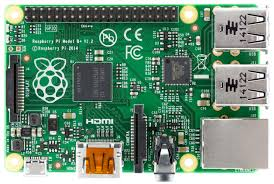
\includegraphics[scale=0.5]{raspi.jpg}
\caption{The Raspberry Pi}
\label{fig:raspberry pi}
\end{figure}

Our system will consist of a wireless network of tiny “client” computers that each control up to 4 lights and are controlled by a central "server" computer, which will automatically send out commands to the clients when it's time to turn on or off.  The central node will run a control program that can be easily accessed via a touch screen, a web browser, or a mobile device, where the user can locally or remotely control each light individually.  Want your lights to turn on at sunset and then dim gradually as the sun rises?  Simple.  Want your lights to flash when you're throwing a party?  Just press a button.  The control interface will allow users to easily set "rules" for what their lights do and when, depending on the time of day, the sun/moon position, and potentially even triggers such as weather conditions or calendar dates.  This system will be easily extensible to potentially control other devices as well, such as garage doors, sound systems, and more.

\begin{figure}[h!]
\centering
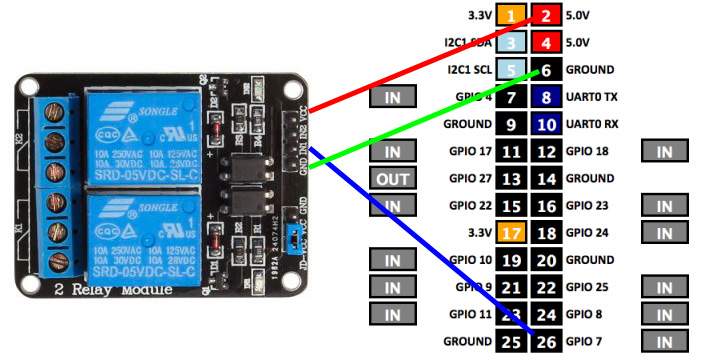
\includegraphics[scale=0.5]{relay.jpg}
\caption{Power relay}
\label{fig:relay}
\end{figure}

To start off, this project will focus on a basic program to run on the server computer that can successfully communicate on/off instructions to the client computers, which then actually turn the lights on/off.  Next, we will need to create an interface for the server node that can be accessed either through the touchscreen or through a web browser/mobile device to actually configure the system.  The final main component will be the implementation of the rule system, which will allow lights to be toggled based on external factors such as sun position.

\begin{figure}[h!]
\centering

\includegraphics[scale=0.5]{wunder.jpeg}
\caption{Wunderground, the API source}
\label{fig:relay}
\end{figure}

What will we be showing at expo?  Simple: the whole thing!  All we need is the system itself and a power source.  Visitors will be able to use the interface to control the lights at the booth!

\end{document}
